%************************************************
\section{Comprehensive Characterization of the Major Presynaptic Elements to the Drosophila OFF Motion Detector}
% \section{Serbe et al., 2016}
\label{sct:manuscript_serbe}
%************************************************

This study mapped the response properties and functional roles of a comprehensive set of input elements to OFF-selective, motion-sensitive T5 cells. The work was published in \textit{Neuron} in February 2016 and highlighted in a News \& Views.

\paragraph{Summary}
Connectomic analysis had identified the four major OFF input cells which together make up more than 90\% of synapses onto T5. Transmedullar units Tm1, Tm2, Tm4, and Tm9 relay signals from lamina projection neurons into the lobula where they contact the dendrites of T5. We used two-photon imaging to monitor calcium signals from each of these cells under visual stimulation. Critically, none of the input elements were themselves selective for direction. This confined the origin of motion detection in the OFF pathway to the dendrites of T5. A broad range of spatial and temporal filters emerged: Tm2 and Tm4 exhibited fast, transient responses to negative contrast change; Tm9 was best approximated as a slow, tonic low-pass filter; Tm1 showed intermediate kinetics. Simulations indicated that this broad filter bank was well suited to extracting motion at relevant time scales. Finally, when blocking cell activitiy individually or in pairs, we observed a broad range of OFF-specific motion deficits. This strongly suggested that each input cell has a particular role to play in detecting motion. None were found to be redundant.

\paragraph{Authors} Etienne Serbe, Matthias Meier (co-first author), \textbf{Aljoscha Leonhardt}, and Alexander Borst.

\paragraph{Contributions} E.S.\ and M.M.\ jointly performed and evaluated all calcium imaging and electrophysiology experiments. \textbf{A.L.}\ performed and evaluated the behavioral experiments. \textbf{A.L.}\ and A.B.\ performed computer simulations. A.B., E.S., and M.M.\ designed the study. E.S.\ and M.M.\ wrote the manuscript with the help of the other authors.

\cleardoublepage

\includepdf[pages=2-last,scale=0.9,offset= 0 40,pagecommand={\thispagestyle{plain}}]{papers/serbe2016}
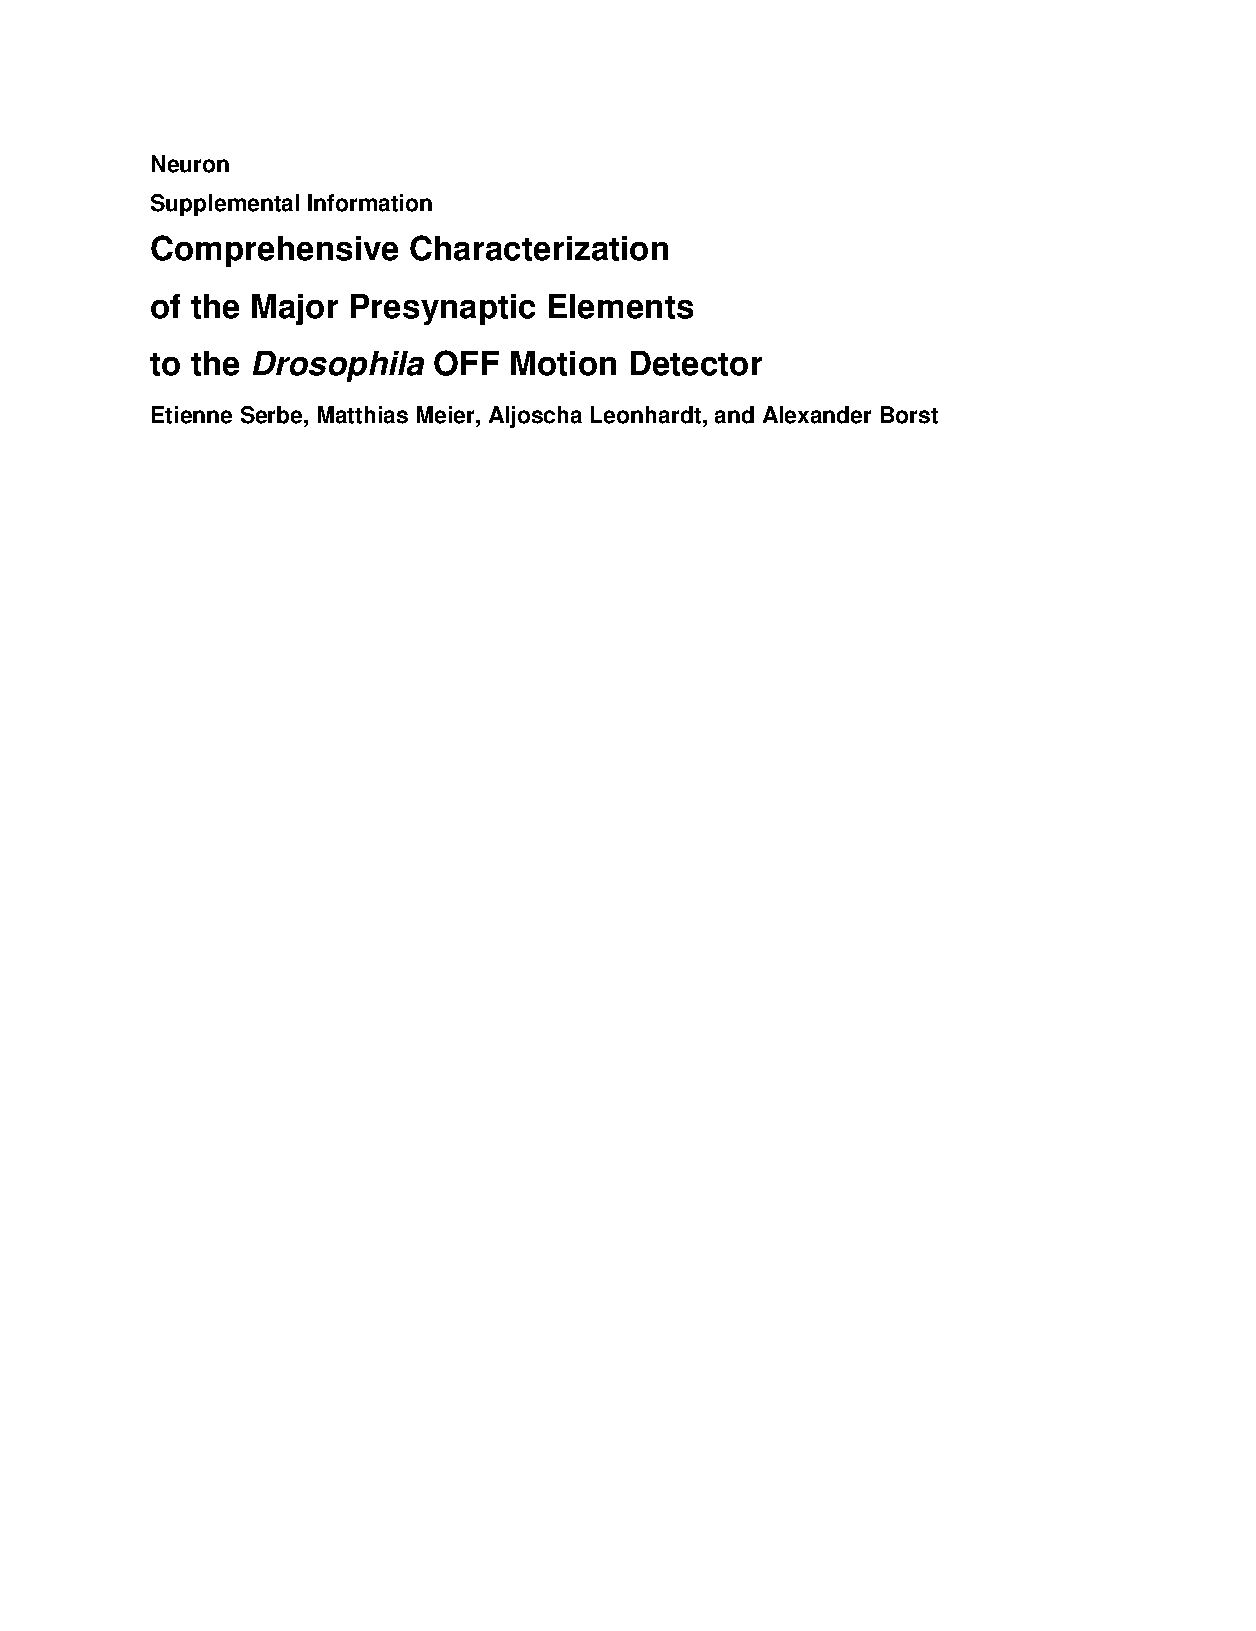
\includepdf[pages=-,scale=0.9,offset= 0 40,pagecommand={\thispagestyle{plain}}]{papers/serbe2016_supplement}